\documentclass[11pt, a4paper]{ctexart} % 使用 ctexart 支持中文

% 引入自定义样式文件
\usepackage{experiment_style}

\begin{document}

% =========================================
% 第 2 题
% =========================================
\begin{problem}{P14. 2}
    利用级数
    \[
        \frac{\pi}{4}=1-\frac{1}{3}+\frac{1}{5}-\frac{1}{7}+\cdots
    \]
    计算无理数 $\pi$ 的近似值。由于交错级数的部分和数列 $S_N$ 在级数的和上下摆动，截断误差将小于第一个被舍弃的项 $\left|a_{n+1}\right|$。试分析：若要使截断误差小于 $10^{-4}$ 或 $10^{-8}$，应该取多少项求和？并分别计算 $\pi$ 的近似值。
\end{problem}

\begin{solution}
    \textbf{实验内容、步骤及结果}

    由于截断误差将小于第一个被舍弃的项 $\left|a_{n+1}\right|$，易编程实现：

\begin{lstlisting}[language=c++]
#include <cmath>
#include <iomanip>
#include <iostream>
#include <vector>

// 判断第 n 项的绝对值是否小于阈值
bool is_term_less_than(int n, double threshold) {
  double term_abs = 1.0 / (2.0 * n + 1.0);
  return term_abs < threshold;
}

// 计算级数前 n 项的和
double calculate_series(int n) {
  double series_sum = 0.0;
  double sign = 1.0;

  for (int i = 0; i < n; ++i) {

    series_sum += sign / (2.0 * i + 1.0);

    sign = -sign; // 每次循环翻转符号
  }
  return series_sum;
}

int main() {
  std::vector<double> expected_trunc_errs = {1e-4, 1e-5, 1e-6, 1e-8};

  std::cout << std::fixed << std::setprecision(10);

  for (double trunc_err : expected_trunc_errs) {
    std::cout << "期望截断误差为: " << trunc_err << "\n";

    int n = 0;
    while (!is_term_less_than(n, trunc_err)) {
      n++;
    }

    std::cout << "需要计算:" << n << "项\n";
    std::cout << "pi的近似值为:" << 4.0 * calculate_series(n) << "\n";
    std::cout << "-----------------------------------\n";
  }

  return 0;
}
\end{lstlisting}

    \textbf{实验结果分析}

\begin{lstlisting}
期望截断误差为: 0.0001000000
需要计算: 5000 项
pi的近似值为: 3.1413926536
-----------------------------------
期望截断误差为: 0.0000100000
需要计算: 50000 项
pi的近似值为: 3.1415726536
-----------------------------------
期望截断误差为: 0.0000010000
需要计算: 500000 项
pi的近似值为: 3.1415906536
-----------------------------------
期望截断误差为: 0.0000000100
需要计算: 50000000 项
pi的近似值为: 3.1415926336
-----------------------------------
\end{lstlisting}

    随截断误差减小，$\pi$ 的估计值越精确，但计算项数也随之增大。
\end{solution}


% =========================================
% P14. 3
% =========================================
\begin{problem}{P14. 3}
    在同一坐标系下，利用 plot 函数画出函数
    \[
        y=\sin x, \quad y_n=\sum_{i=0}^n(-1)^i \frac{x^{2 i+1}}{(2 i+1)!}, \quad(n=2,5,10)
    \]
    的图形，并加标注说明各条曲线的含义。
\end{problem}

\begin{solution}
    \textbf{实验内容、步骤及结果}

\begin{lstlisting}[language=c++]
#define _USE_MATH_DEFINES
#include <iostream>
#include <vector>
#include <cmath>
#include <fstream>

// ---------------------------------------------------------
// 递推公式: Term_i = Term_{i-1} * (-x^2) / ((2i)*(2i+1))
// ---------------------------------------------------------
std::vector<double> taylor_series(const std::vector<double>& x_vals, int n) {
    std::vector<double> result(x_vals.size(), 0.0);
    
    for (size_t k = 0; k < x_vals.size(); ++k) {
        double x = x_vals[k];
        double term = x;
        double sum = term;
        
        for (int i = 1; i <= n; ++i) {
            term *= (-x * x) / ((2.0 * i) * (2.0 * i + 1.0));
            sum += term;
        }
        result[k] = sum;
    }
    return result;
}

int main() {
    // 1. 生成 x 的数据点
    int num_points = 80;
    double x_start = -2.0 * M_PI;
    double x_end = 2.0 * M_PI;
    double step = (x_end - x_start) / (num_points - 1);
    
    std::vector<double> x, y_true, y_2, y_5, y_10;
    
    for (int i = 0; i < num_points; ++i) {
        double current_x = x_start + i * step;
        x.push_back(current_x);
        y_true.push_back(std::sin(current_x)); // 真实的 sin(x)
    }

    // 2. 计算不同阶数的泰勒展开
    y_2 = taylor_series(x, 1);   // n=1 (计算到 x^3)
    y_5 = taylor_series(x, 5);   // n=5 (计算到 x^11)
    y_10 = taylor_series(x, 10); // n=10 (计算到 x^21)

    // 3. 将计算结果输出到 CSV 文件，供 Python 画图使用
    std::ofstream file("q3_data.csv");
    if (!file.is_open()) {
        std::cerr << "无法创建文件!" << std::endl;
        return 1;
    }
    
    // 写入表头
    file << "x,y_true,y_2,y_5,y_10\n";
    // 写入数据
    for (size_t i = 0; i < x.size(); ++i) {
        file << x[i] << "," << y_true[i] << "," 
             << y_2[i] << "," << y_5[i] << "," << y_10[i] << "\n";
    }
    file.close();

    return 0;
}
\end{lstlisting}

\begin{lstlisting}[language=Python]
import math
import numpy as np
import matplotlib.pyplot as plt
from decimal import Decimal, getcontext

getcontext().prec = 50
x = np.linspace(-2 * np.pi, 2 * np.pi, 80)
y = np.sin(x)

def taylor_series(x, n):
    result = np.zeros_like(x, dtype=np.float64)
    for i in range(n + 1):
        result += ((-1) ** i) * (x ** (2 * i + 1)) / float(Decimal(math.factorial(2 * i + 1)))
    return result

y_2 = taylor_series(x, 1)
y_5 = taylor_series(x, 5)
y_10 = taylor_series(x, 10)

plt.plot(x, y, label='y=sin(x)', color='blue')
plt.plot(x, y_2, label='y_2', color='green')
plt.plot(x, y_5, label='y_5', color='red', linestyle='--')
plt.plot(x, y_10, label='y_10', color='orange', linestyle='-.')

plt.ylim(-1.5, 1.5)

ax = plt.gca()
ax.spines['left'].set_position('center')
ax.spines['bottom'].set_position('center')
ax.spines['right'].set_color('none')
ax.spines['top'].set_color('none')
ax.xaxis.set_ticks_position('bottom')
ax.yaxis.set_ticks_position('left')

plt.legend()
plt.show()
\end{lstlisting}

    \textbf{实验结果分析}
    
    % 注意：确保存放图片的 assets 文件夹在 main.tex 同级目录下
    \begin{center}
        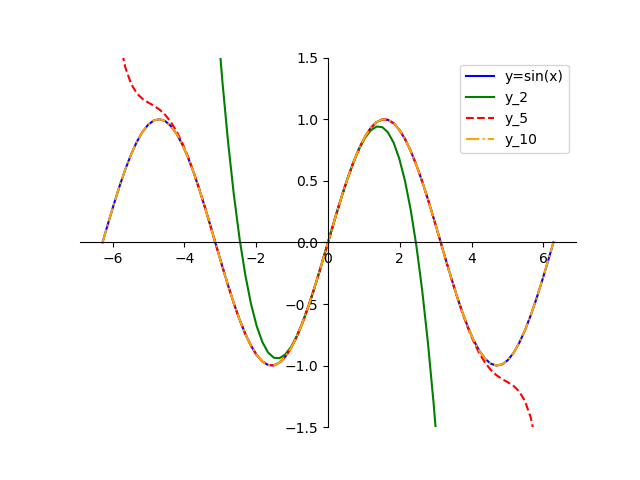
\includegraphics[width=0.8\textwidth]{assets/fig1.png}
    \end{center}

    当 $x\to 0$ 时，用泰勒展开近似 $\sin x$ 的截断误差较小。随着 $|x|$ 增大，截断误差越明显。
\end{solution}


\end{document}
